\section{Research model} \label{research_model}

Figure \ref{fig_conceptual_framework} depicts the overall conceptual research framework.
The artifact is the research context. It is a fully functional commerce Restful API with
ASP.NET (v6) and C\# (v10). The research aims to test the cause-and-effect relationship
between Clean Architecture (independent variable) and the evolvability of the C\#
artifact.

The Normalized Systems Theorems do not affect Clean Architecture as an independent
variable. Instead, it will affect the design of the artifact. Previous research and case
studies have already shown that Normalized Systems affect the evolvability of software
artifacts by using a prescribed modular design, mitigating combinatorial effects.
Normalized Systems Theorems is the control variable in the conceptual framework.

Since we are trying to prove the convergence of Normalized Systems and Clean
Architecture the Modular architecture will be compared with the design of Normalized
Systems. Therefore, Modular Architecture is positioned as the Mediator variable in this
conceptual framework.

\begin{figure}[!ht]
    \centering
    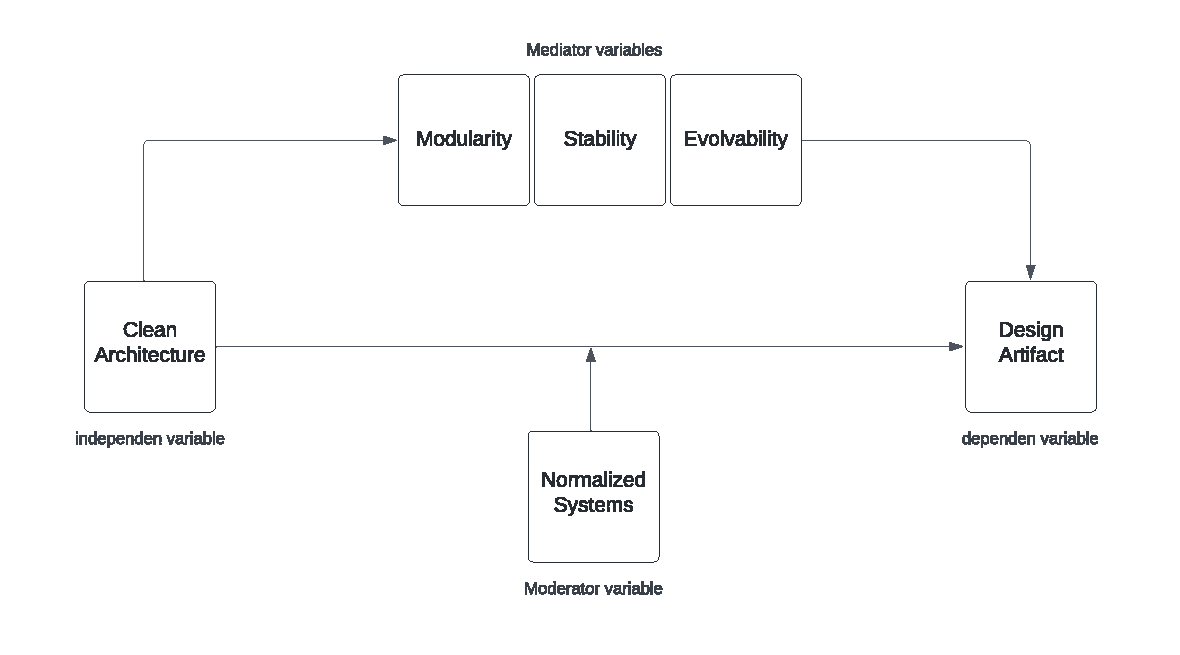
\includegraphics[width=1\textwidth]{Figures/conceptual_framework}
    \caption[Overall conceptual framework]{Overall conceptual framework}
    \label{fig_conceptual_framework}
\end{figure}
